\documentclass[11pt]{article}
\usepackage[a4paper, total={6.5in, 9in}, headheight=14.5pt]{geometry}

\geometry{letterpaper}
\geometry{portrait}
\usepackage{multicol}
\usepackage{hyperref}
\usepackage[parfill]{parskip} 
\usepackage{times}
\usepackage{wrapfig}
\usepackage[utf8]{inputenc}
\usepackage[english]{babel}
\usepackage{physics}
\usepackage{float}


% Math packages
\usepackage{amsmath}
\usepackage{amssymb}
\usepackage{booktabs}

% For Line spacing
\usepackage{setspace}              % Load the setspace package
\doublespacing                     % Make the entire document double-spaced


% For including graphics
\usepackage{graphicx} % allows figures to be added to the document
\usepackage{pifont}

% For referencing and bibliography
\usepackage{hyperref} % add hyperlink and hypertext capabilities 
\usepackage[]{natbib}
\usepackage{fancyhdr}

% 3. Change the page style to fancy
\pagestyle{fancy}

\fancyhf{}

\fancyhead[L]{H. Nachman}       % Left Header
\fancyhead[C]{LAT Pointing Jitter Simulations}                   % Center Header
\fancyhead[R]{\thepage}               % Right Header (Dynamically shows current Section)
\renewcommand{\headrulewidth}{0.4pt}


\setcitestyle{authoryear, round}

\bibliographystyle{apalike}

% For color text
\usepackage{xcolor}
\begin{document}
%  NOW you can start changing stuff!

\title{LAT Pointing Requirements
\thanks{
Correspondence to:  henry.nachman@utexas.edu}
}


\author{H. Nachman\\
{\it  University of Texas at Austin}\\
{\it Austin, Texas}\\
 }

% \maketitle

% \def\mnu{m_\nu}
\def\neff{$N_{\rm eff.}$}
\def\LCDM{$\Lambda$CDM}


\section{Overview}
The basic goal of this project is to determine what the pointing requirements are for various SO LAT science goals, and evaluate whether these goals have been achieved (and ultimately, if not, explore what elements of pointing are limiting us). Some of the framework for how this project will proceed are based on Elisa Russier's talk at the F2F 2026. 

The goal can be thought of in a sentence such as:
\begin{quotation}
    {\bf X} must be known to within {\bf a\%} to avoid biasing {\bf Y} by more than {\bf b\%}.
\end{quotation}

In the case of pointing, this might look like:
\begin{quotation}
    Pointing must be known to within 5 arcsec to avoid biasing {$\sigma_8$} by more than {2\%}. (these are random numbers just for example)
\end{quotation}

Where do each of these components come from? 

\subsection{Expected (simplified) Pipeline:}
\begin{enumerate}
    \item Simulate pointing errors in maps: \begin{itemize}
        \item TOAST - TOD based simulation framework. Would allow me to consider pointing errors in maps, but might be more complex than needed.
        \item SMARTIES - Map-space simulation, should allow me to consider pointing errors in maps - less documentation.
    \end{itemize}
    \item Maps to data product, primarily power spectra:\begin{itemize}
        \item Pass simulated maps through realistic pipelines to achieve realistic power spectra.
        \item What different `data products' (eg. types of power spectra) are needed to perform step 3.
    \end{itemize}
    \item Analyze data product to put constraints on parameters:\begin{itemize}
        \item Which means I need to understand how to go from 'data product' (power spectra, etc.) to parameter constraints - potentially different for each parameter.
        \item Is this via MCMC parameter estimation techniques like CosmoMC/Cobaya + CAMB/CLASS that will give me confidence intervals for parameters given a single pointing realization?
        \item Or more simply, once I have the parameter constraints -- one with no pointing errors and one with pointing errors -- I can compare the two to see how the addition of pointing errors impacts the product. 
		% \item Eg. How does the matter power spectrum change with pointing errors, and how does this change on the matter power spectrum impact our ability to measure Neff
    \end{itemize}
\end{enumerate}


\subsection{How to start / guidance I need:}
\begin{enumerate}
    \item Figure out how to simulate maps + include pointing errors (jitter beams) into maps: \begin{itemize}
        \item If the path is TOAST - then I think I have what I need to at least get started with sims but it might take a bit of figuring out before I have maps that I can use.  
        \item If the path is SMARTIES - Who can I talk to about SMARTIES because I have not yet found much documentation. Using SMARTIES will require I have a better understanding of how exactly different sources of pointing errors impact maps - simple `beam smoothing', or more complex situations.
        \item {\bf What sort of mapmaking simulation framework should I be using/starting on? And what resources are there (people/documentation/examples) to help facilitate me learning this framework?}
    \end{itemize}
    \item How do I determine the uncertainty in a parameter - this is very new to me? \begin{itemize}
        \item {\bf What does the parameter estimation (and uncertainty estimation) pipeline look like? How should I behind to approach this?}
        \item {\bf Which cosmological parameter should I focus on? Map science vs transient science?}
        % \item Do I for now, pick 1 cosmological parameter?
        \item Do we know which case(s) have the strictest pointing needs? 
        \item Map science vs transient science? Does transient science analysis rely solely on the static pointing model or can it use point-source corrections? 
        \item How does one go from a map to a parameter constraint? CosmoMC/CLASS/CAMB with MCMC parameter estimation methods (as in ACT)?

    \end{itemize}
\end{enumerate}

\subsection{Other questions I have}
\begin{itemize}
    \item 
\end{itemize}
\pagebreak

\subsection{Science Goals}

The enhanced Large Aperture Telescope (LAT) has a number of science goals across cosmological, astrophysical, and particle physics fields, and stemming from a variety of different measurement/analysis channels. Understanding how pointing impacts the science results requires pairing each science goal with its respective analysis method. For example, \cite{abitbol_simons_2025} states the enhanced LAT will place a constraint on the number of relativistic species $\sigma(N_\text{eff}) = 0.045$. This constraint is largely set by imprints in the small-scale damping tail of the CMB temperature and polarization anisotropy power spectra. Thus, to determine how pointing impacts this constraint on $N_\text{eff}$, one would need to simulate how changes in pointing impact the power spectra (in this case we might predict that pointing errors that express themselves as smoothing of the beam would effective limit/increase uncertainty on the smallest scales of the power spectrum).



\begin{table*}[h!]
    \center
\caption[Simons Observatory Surveys]{Summary of Enhanced Science Goals from SO LAT Survey\textsuperscript{a}}  \footnotesize
\begin{tabular}{ l | c | c | c | l }
\hline
\hline

 & Current\textsuperscript{b} & {\bf SO} & Using Rubin, & Reference \\
 &                            & {\bf 2025--2034}             & DESI, or {\sl Euclid}    & \\
\hline
\hline
{\bf Primordial perturbations}  &&&&\\
\hline
$n_s$ & 0.004 & 0.002 &  - & Shandera 2019\\%\citet{shandera/etal:2019} \\
 $e^{-2\tau}\mathcal{P}(k=0.2\,\rm{Mpc^{-1}})$ & 3\% & 0.4\% &  - & Slosar 2019\\%\citet{slosar/etal:2019b}\\
$f^{\rm local}_{\rm{NL}}$ &  5&  1 & \ding{51} & Meerburg 2019\\%\citet{meerburg/etal:2019}\\
\hline
{\bf Relativistic species} &&&&\\
\hline
$N_{\rm eff}$ &  0.2 & $0.045$  & - & Green 2019\\%\citet{green/etal:2019}\\
\hline
{\bf Neutrino mass\textsuperscript{c}} &&&&\\
\hline
$\sum \mnu$ (eV, $\sigma(\tau)=0.01$) & 0.1 &  0.03 & \ding{51}  & Dvorkin 2019\\%\citet{dvorkin/etal:2019} \\
$\sum \mnu$ (eV, $\sigma(\tau)=0.002$) & &   0.015  & \ding{51} &\\
\hline
{\bf Accelerated expansion} &&&&\\
\hline
$\sigma_8(z=1-2)$& 7\%& 1\% & \ding{51} & Slosar 2019\\%\citet{slosar/etal:2019}\\
\hline
{\bf Galaxy evolution} &&&&\\
\hline
$\eta_{\rm feedback}$ & 50--100\% & 2\% & \ding{51} & Battaglia 2019\\%\citet{battaglia/etal:2019}\\
$p_{\rm nt}$  & 50--100\% & 4\% & \ding{51} & Battaglia 2019\\%\citet{battaglia/etal:2019}\\
\hline
{\bf Reionization } &&&&\\
\hline
$\Delta z$ & 1.4 & 0.3 & - & Alvarez 2019\\%\citet{alvarez/etal:2019}\\
$\tau$ & 0.007 & 0.0035 & - & Alvarez 2019\\%\citet{alvarez/etal:2019}\\
\hline
{\bf Cluster catalog} & 4000 & 33,000 & \ding{51} &\\
{\bf AGN catalog} & 2000 & 96,000 & - &\\
\hline
{\bf Galactic science} &&&&\\
\hline
{Molecular cloud B-fields} & 10s & $>860$ & - & SO 2022 GS\\%\citet{SO_2022_Galactic_Science}\\
{$\sigma (\beta_\mathrm{dust})$} & 0.02  & $0.005$ & - & SO 2022 GS\\%\citet{SO_2022_Galactic_Science} \\
\hline
{\bf Solar System Science } &&&&\\
\hline
{Distance limit for 5 $M_\oplus$ Planet 9} & 500 AU &  900 AU  & \ding{51} & Fienga 2020\\%\citet{Fienga2020} \\
{Asteroid detections} &  &  $\sim10,000$  &  &\\
\hline
{\bf Transient detection } &&&&\\
{\bf \,\,\, distance} &&&&\\
\hline
{Long GRBs, on-axis} &  &  
1300 Mpc  & - &\\
{Low-luminosity GRBs} &  & 
70--210 Mpc  & - &\\
{TDEs, on-axis} &  & 670 Mpc  & - &\\
\hline
\end{tabular}
% \begin{tablenotes}
% \item \textsuperscript{a}  Projected 1$\sigma$ errors computed with standard methodology as in \\%\citet{so_forecast:2019}, scaled to account for the improved noise from the enhanced infrastructure described in Sec.~\ref{sec:infrastructure} (see Appendix~\ref{app:sensitivities}).  Galactic science forecasts are computed as in \\%\citet{SO_2022_Galactic_Science}. \\%\citet{so_forecast:2019} describes our methods to account for noise properties and foreground uncertainties. We adopt ``goal'' noise levels for the SO LAT in these forecasts.  A 20\% end-to-end observation efficiency is used, matching that typically achieved in Chile \citep[as also assumed in][]{so_forecast:2019}. We assume the {\it Planck} data are included throughout. External data listed in the fourth column are those necessary to achieve the forecasted precision on each individual science target; for the cluster catalog the external data are needed only for obtaining redshifts.  Note that the time-domain science forecasts are new to this work, as this topic was not considered in the nominal SO science goals forecasting~\citep{so_forecast:2019}. 
% \item \textsuperscript{b} Primarily from \PLANCK\ \citep{planck_cosmo:2018}. We anticipate constraints from existing ground-based data to improve on the ``current'' limits in the near future.  These constraints are expected to lie between the ``current'' and SO levels.
% \item \textsuperscript{c} The forecast precision on $\sum m_\nu$ is highly sensitive to the projected error bar on $\tau$, and thus we provide two forecasts here (see Sec.~\ref{subsec:LSSmapping}).
% \end{tablenotes}
\label{tab:goals}
\end{table*}



\subsection{Sources of (LAT) Pointing Error}

\begin{itemize}
    \item Azimuth, Elevation, Corotator encoder offsets
    \item Axis misalignment between corotator, mirrors, elevation space and the LATR
    \item Physical elevation sag of mirrors with gravity
    \item Tilts of the entire platform
    \item Thermal fluctuations
    \item Distortions in focal plane from off-axis mirror design
\end{itemize}




\citep{abitbol_simons_2025} \citep{aiola_atacama_2025}
% \section{Simulating Time-Ordered Data}

Simulation of the TOD from a telescope scan is done in TOAST. TOAST works by generating data from a simulated scan of a sky. Adjustments to either the TOD or the telescope properties (such as pointing) is done via apply operators. To simulate pointing errors I need to create a new pointing error operator, scan a simulated CMB map, then proceed with parameter estimation.

Before I can implement pointing errors, I need a way to qualify, and quantify, the efficacy of my operator. While I could scan a basic simulated CMB map, I am not confident I would be able to tell if my operator is doing exactly what I want it to do. Instead I want to scan a blank map with a single point source. In this way, the effects of my pointing errors will be more evident. To create this map I will use \verb+healpy+.

I also need a way of recreating maps from the TOD. Both \verb+TOAST+ and \verb+sotodlib+ have methods for this.



\pagebreak

% \section{Updates}
{\bf Overview}\\
In brief, thus far, I have made TOAST-style pointing offset and pointing jitter operators which I have been able to run through simple (non-LAT specific) TOAST simulations. From these I can run a basic filter bin or ml mapmaker and can confirm that a simulated point source gets 'messed up'. I can also confirm that the operators adjust my pointing in the way I expect and I can run some basic beam statistics analysis on the output map (although the maps aren't themselves realistic so this was just for demonstration purposes)
I have added these operators to a local dev version of TOAST and SOTODLIB for running with the toast\_so\_sim cli so that I can model a more realistic LAT camera. This is sort of where I have hit a little wall as I have struggled to figure out how/where exactly to add the execution of my operator in the sim workflow. My toast\_so\_sim appears to run my custom operator and apply the pointing error, but the output maps are largely identical to maps with no pointing errors. I presume this is an error in how I have incorporated the custom operator into the larger simulation framework but I am still figuring that out. 

Some of my questions are specific to how to implement this in TOAST (and might not need a meeting of all of us). I also have some bigger picture questions that we should probably discuss as a group such as:

\begin{itemize}
    \item How should I be quantifying the impact of pointing errors? I was thinking I could simulate a scan of a point source and then calculate some beam statistics on the resulting map. If so, what point source? What beam stats do we care about? I presume there is existing code to do some of this for LAT beams, which code should I be using?
	\item How specifically do we want to model pointing jitter? I am currently using a sinusoidal error with gaussian noise (specifying the noise rms) as a starting point, but we should figure out if that is how we want to do things?
	\item Once I can confirm that my operator is working as intended, how should I proceed with simulating CMB observations towards the ultimate goal of using that simulated data for producing 'science'.
\end{itemize}

{\bf 2026-10-12 and 2026-10-13}\\

Today I added the basic pointing offset operator in the same way that I tried to add the pointing jitter operator as the effects of a pointing offset operator should be easier to observe than a simple pointing jitter. Claude gave me some advice as to how to properly add the new operators and make my operator more amenable to a generic TOAST sim. These changes include:
\begin{itemize}
    \item Making the operator have the option to output to a new shared key instead of overwriting the default pointing. This is so that the mapmaking scripts do not use the modified pointing, but rather the nominal pointing when trying to achieve a mapmaking solution.
    \item Making new \verb+apply_pointing_offset+ functions that can be called from the \verb+so_sim/simulate_data+ function. 
\end{itemize}

At least now I can confirm that the pointing offset operator is in fact being called, and that it is modifying the pointing as expected, as shown in the following figure.
\begin{figure}[h!]
    \centering
    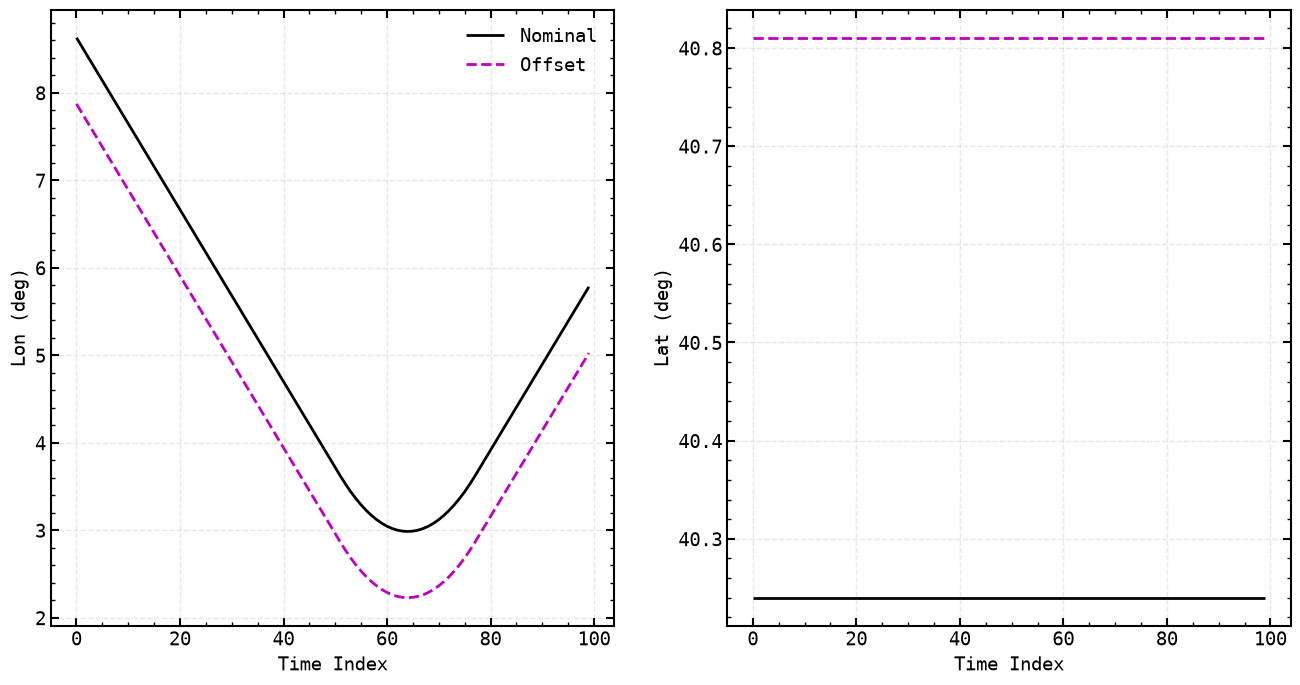
\includegraphics[width=0.8\textwidth]{Updates/figures/offset_lonlat.png}
    \caption{Pointing offset operator in action}
\end{figure}

But when I try and run the mapmaker once without offset, and once with, I still get nearly identical maps.

\begin{figure}[h!]
    \centering
    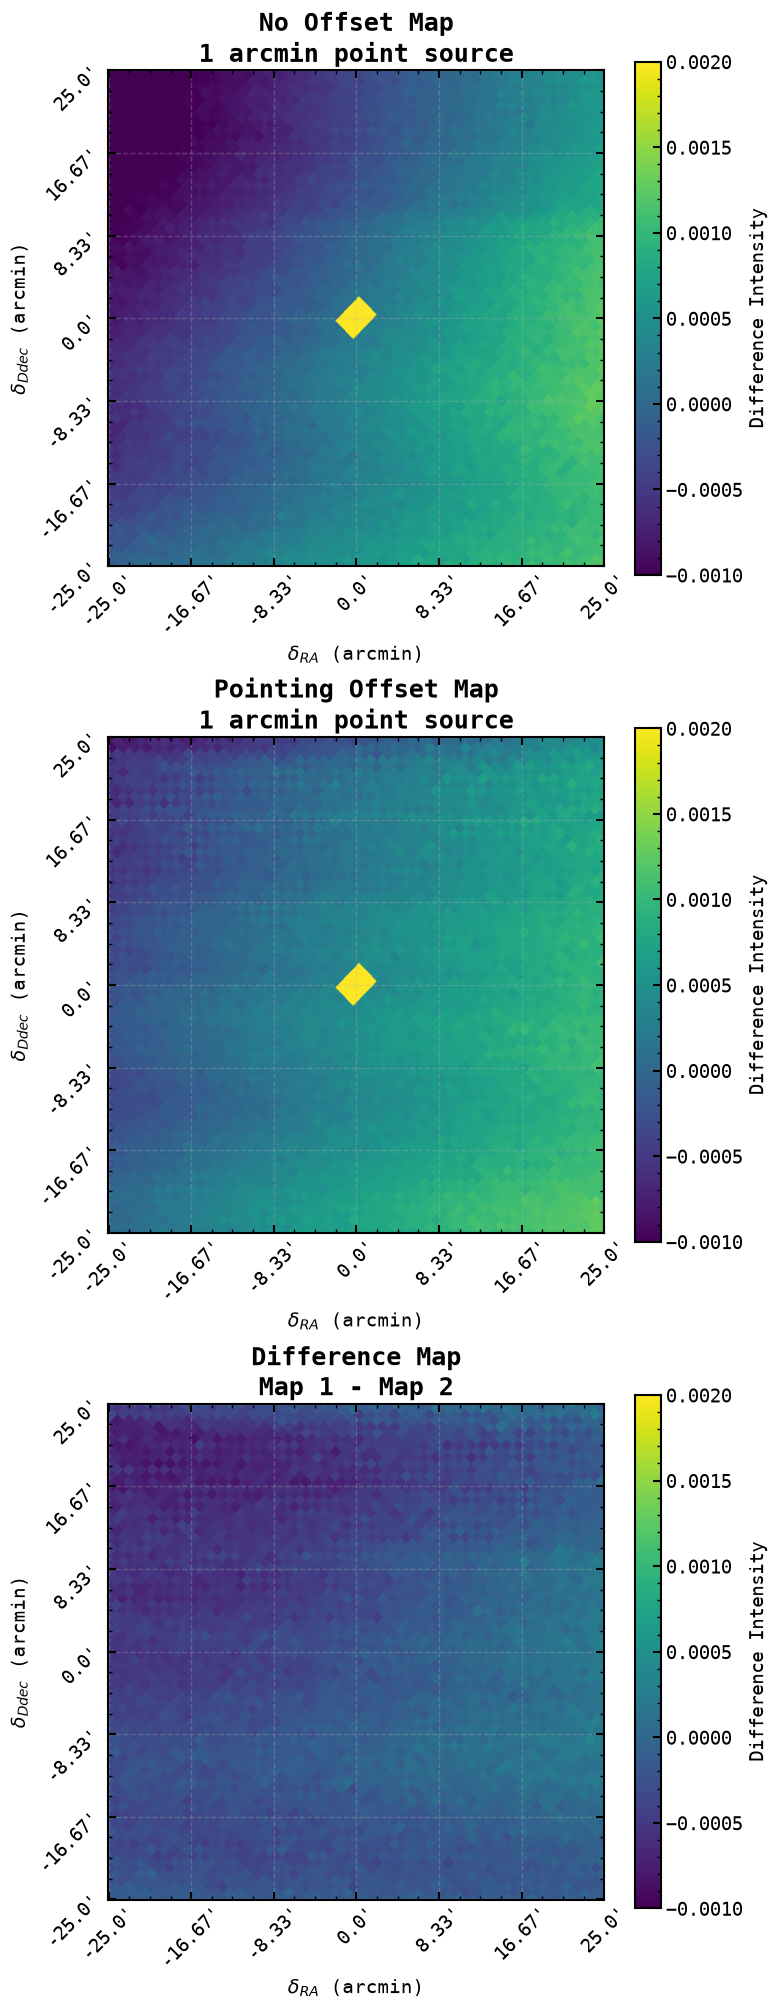
\includegraphics[width=0.5\textwidth]{Updates/figures/offset_diff_maps.png}
    \caption{Pointing offset operator in action}
\end{figure}

I am also a little concerned by the fact that my maps are not producing a sort of Airy disk pattern that I would expect from simulating a point source. I don't know if this is because of the way I am injecting a point source into my input maps, or because of how I am running the mapmaker, or something else. 
{\bf 2026-10-11}\\

Adding the custom operator is unfortunately non-trivial. Just calling the operator argument with something like \verb+--pointing_jitter.enable+ does not inherently tell the sim how and when to run the operator.

Based on some trial and error (and lots of debugging print statements) it seems like code need to be added to the following places:

With this in place, I reran the sims with a 2 arcmin source and pointing jitter of $\delta_{az}, \delta_{el} \sim 0.0001$ and $\delta_{az}, \delta_{el} \sim 0.001$.

Unfortunately, the output maps looks identical as shown by the following difference plot.

It is a little hard to tell if this is because the pointing jitter operator is not working, not in the right place in the code, or simply not having a level of impact strong enough to notice in this sort of map.
{\bf 2026-10-08}\\

I have spent the better part of the last 10 days trying to figure out how to run a more realistic LAT toast sim. Here is what I have learned:
\begin{enumerate}
    \item A realistic SO TOAST sim is largely run through the use of the command line interface (CLI) from the sotodlib module (\verb+toast_so_sim+). The CLI has a huge (thousands) of possible command line arguments to specify which operators to apply and operator parameters. This interface can also likely take config files to ensure reproducibility but I haven't really played around with that.
    \item While adding the new pointing jitter operator to the list of possible operators to call in the CLI is fairly straightforward, it is not clear how/where to include calling the new operator in the pipeline of a toast sim.
    \item The large number of arguments are not really accompanied by clear instructions indicating which operators need to be specified for a particular type of simulation. For instance, I have been trying to scan a solar system object (SSO) for a semi-realistic simulation of a point-source. Turns out defining the SSO in your schedule does not make toast actually simulate the source, to do this, you need to enable the \verb+--sim_sso.enable+ argument. But this argument seems to also require other arguments to be specified. What those arguments are, and what they should be set to is not clear (for example, what beam file should I specify).
    \item Running from a CLI makes many interactive things like plotting the impact of my operator much more difficult.
\end{enumerate}

Before I can do anything, I need to make sure that running the toast sim CLI actually pull from my custom code (since my code is not yet incorporated into the greater TOAST, sotodlib packages). The instructions for doing this are mostly documented on the SO wiki page for using NERSC. In brief, the steps are:
\begin{enumerate}
    \item Create a custom conda environment.
    \item Install the sotodlib and toast packages from source.
\end{enumerate}

Once this is done, the new operator must be added to the list of available operators for \verb+toast_so_sim+



Because I did not want to deal with trying to figure out how to use the toast SSO method, I just had toast spit out the RA/Dec of where Mars was from its schedule, then adjusted my input maps to have a point source at that location. 

\begin{figure}[h!]
    \centering
    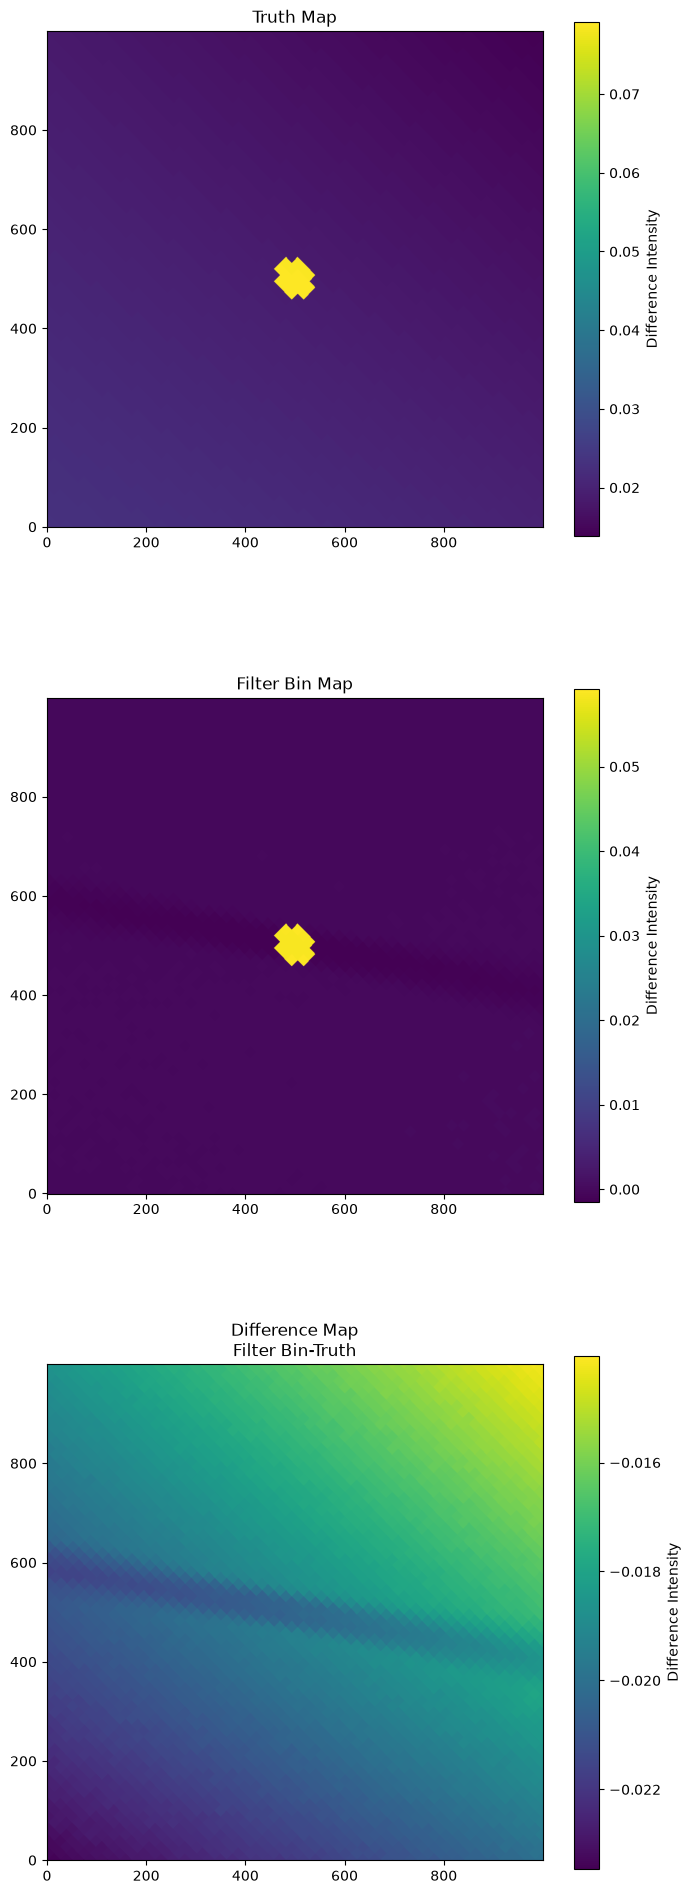
\includegraphics[width=0.5\textwidth]{Updates/figures/diff_map_2arcmin.png}
    \caption{Difference between input map and filter bin scan.}
    \label{fig:diff_map}
\end{figure}

To test that the CLI method was working, I ran a toast sim of my fake 'Mars' map without any pointing jitter. It took me a minute to get the inputs correct so that it would actually scan my custom map, and also run a filter bin mapmaker on the resulting TOD. After some trial and error, I was able to get the following map.

{\bf 2026-09-30}\\
I have a simple simulation pipeline that can make a toast simulation scanning a custom map, with or without pointing jitter. Then run a ml mapmaker or a filter bin mapmaker on the resulting TOD. 

The input map looks like this - for a 10arcmin source:

\begin{figure}[h!]
    \centering
    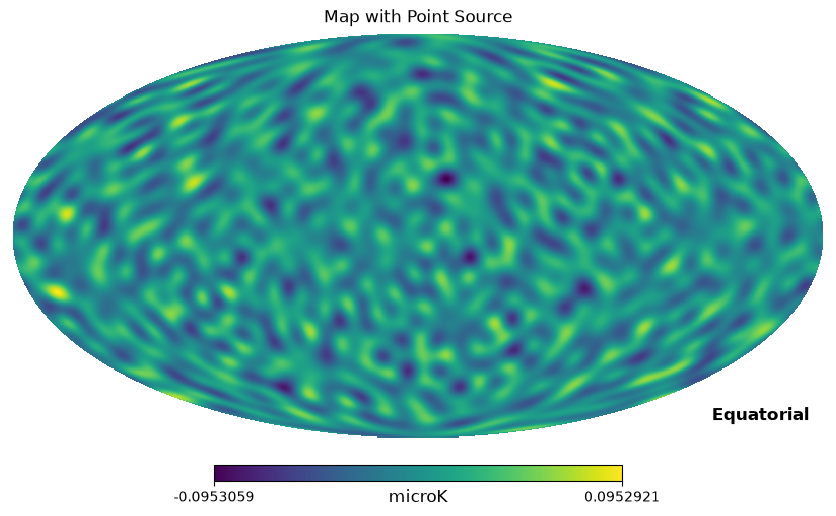
\includegraphics[width=0.75\textwidth]{Updates/figures/simple_map_wsource.png}
    \caption{Input map for the simulation.}
    \label{fig:input_map}
\end{figure}

\begin{figure}[h!]
    \centering
    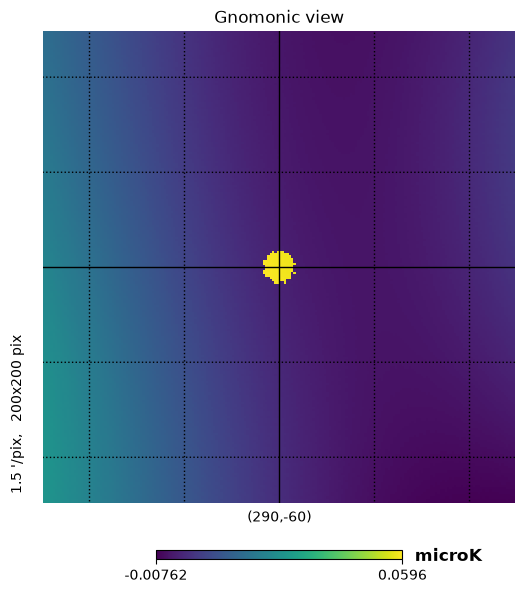
\includegraphics[width=0.75\textwidth]{Updates/figures/simple_map_wsource_gnom.png}
    \caption{Input map for the simulation - gnomonic projection of the source.}
    \label{fig:input_map_gnom}
\end{figure}


The toast sim also produces some pointing visualizations to confirm that the pointing jitter is being applied as expected.

\begin{figure}[h!]
    \centering
    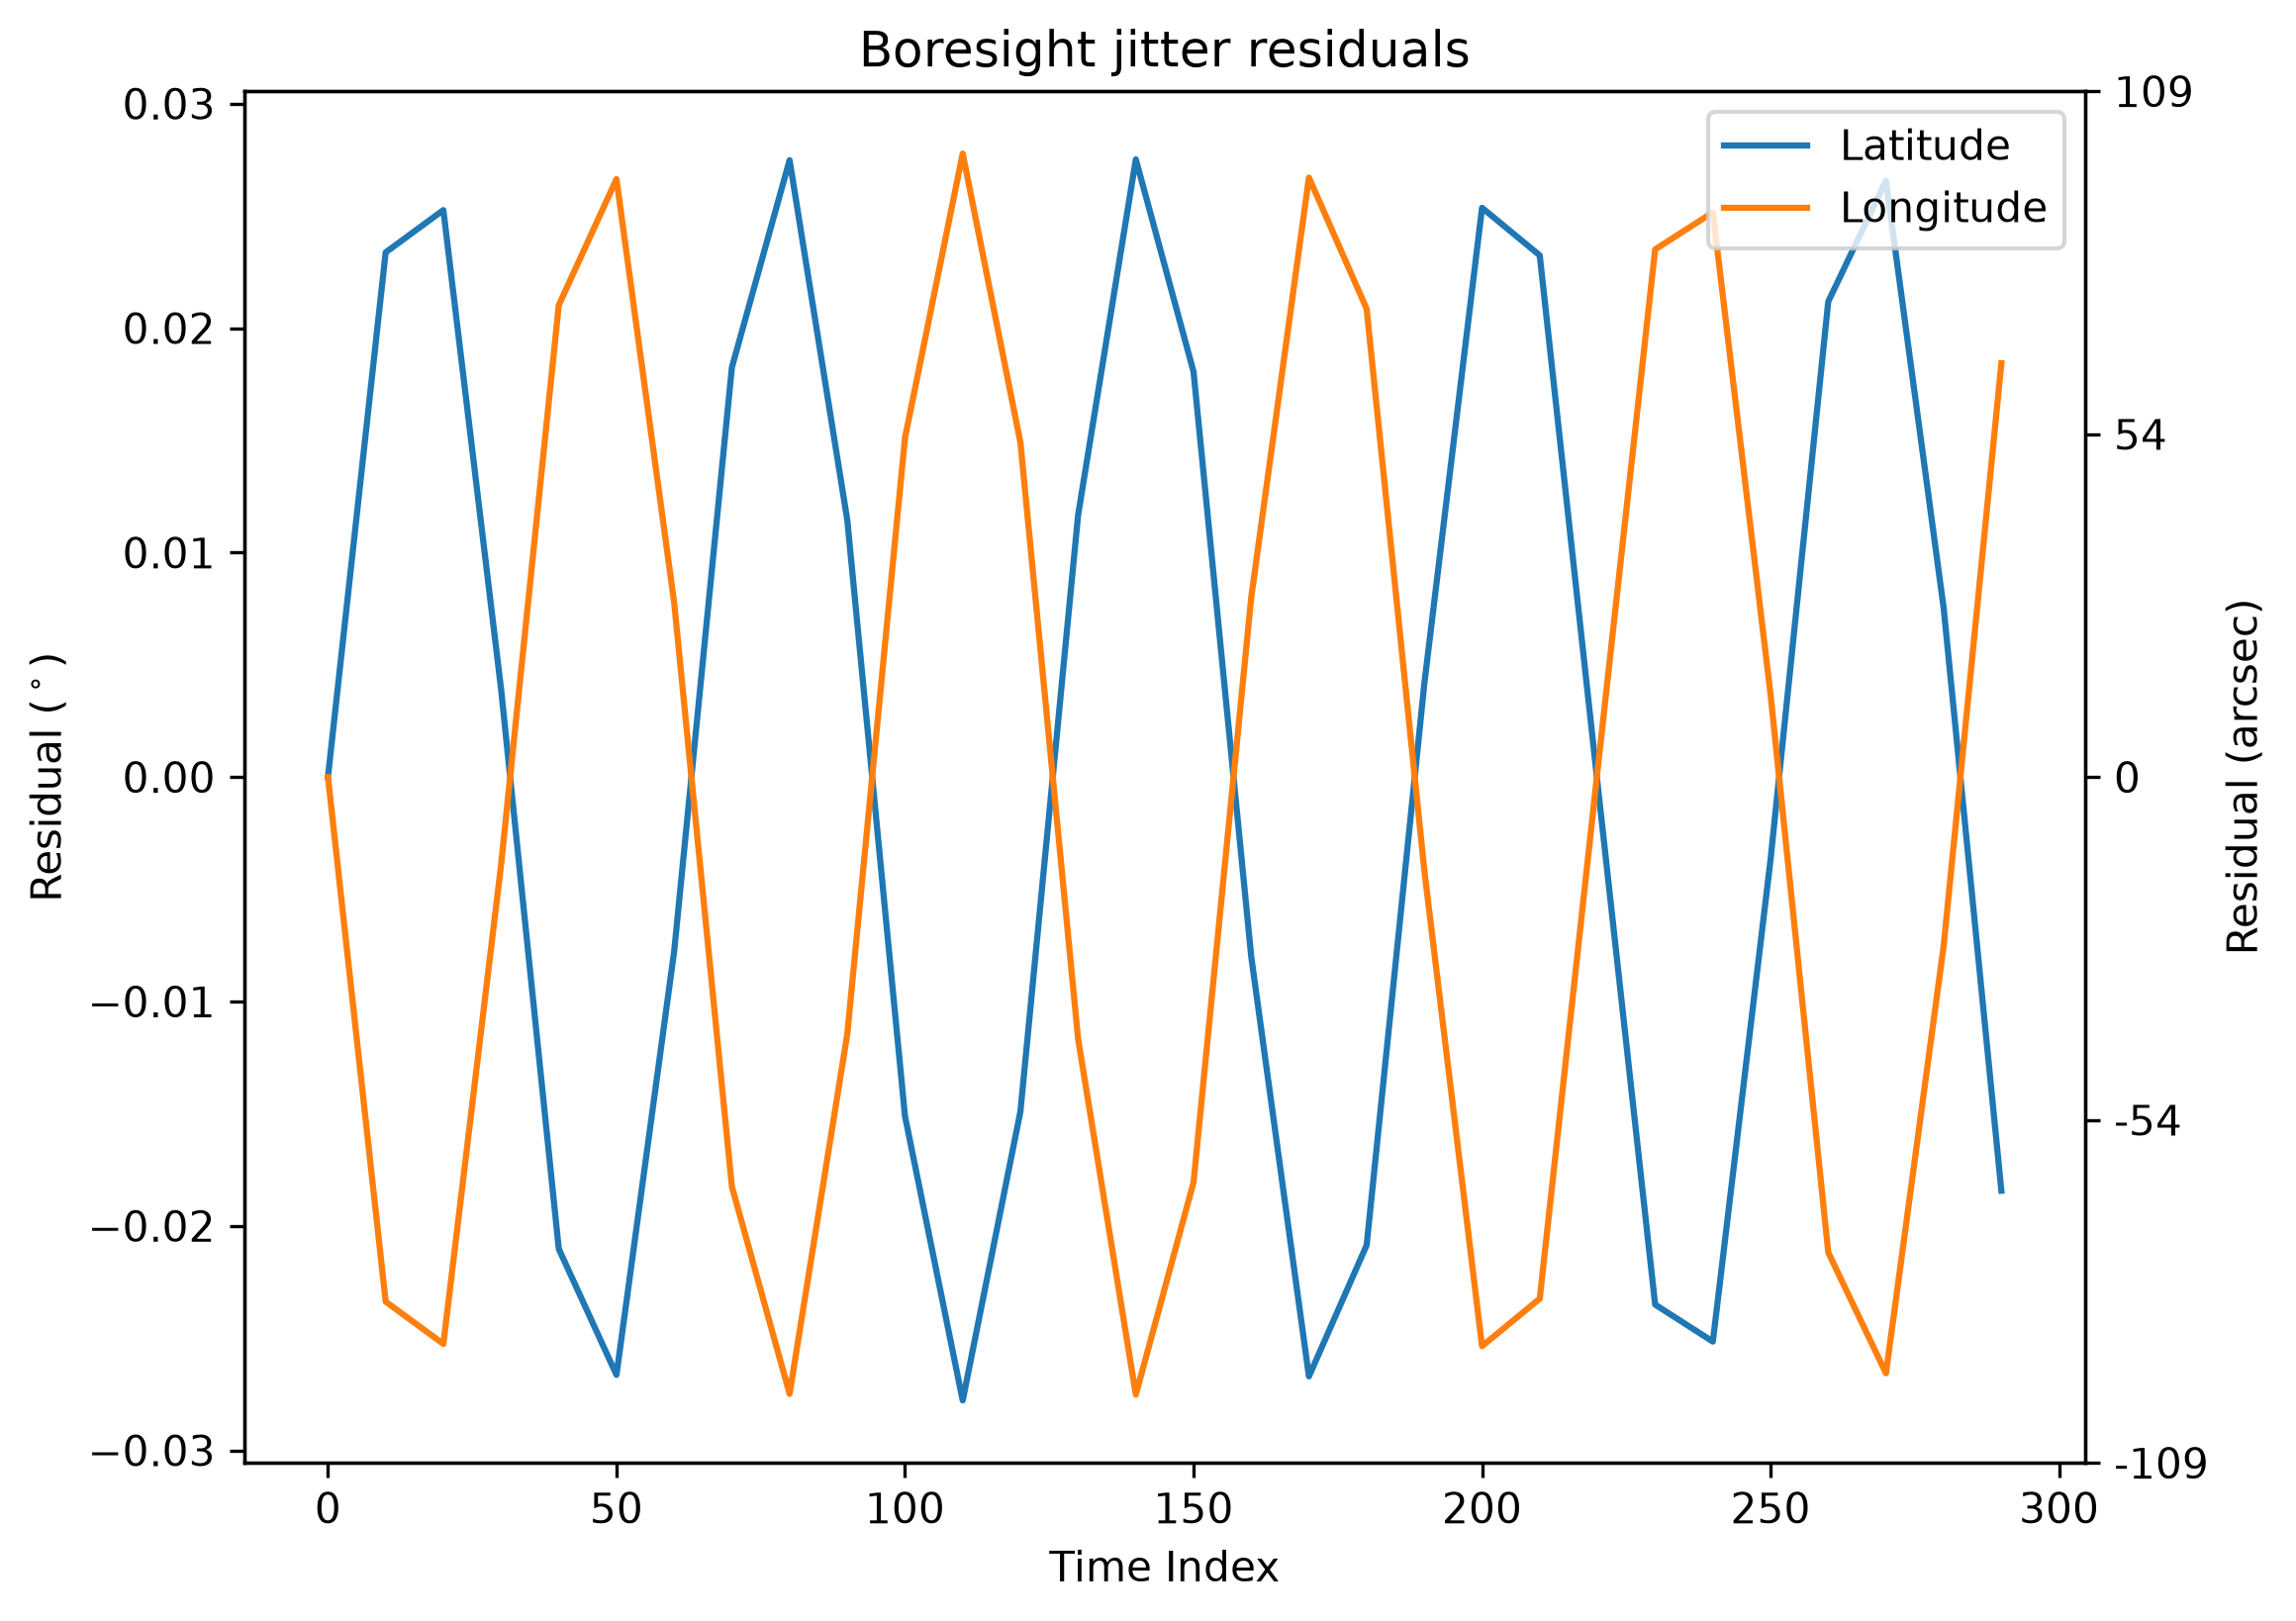
\includegraphics[width=0.75\textwidth]{Updates/figures/boresight_residuals.png}
    \caption{Pointing jitter boresight residuals.}
    \label{fig:boresight_res}
\end{figure}

This can be viewed in 3D:

\begin{figure}[h!]
    \centering
    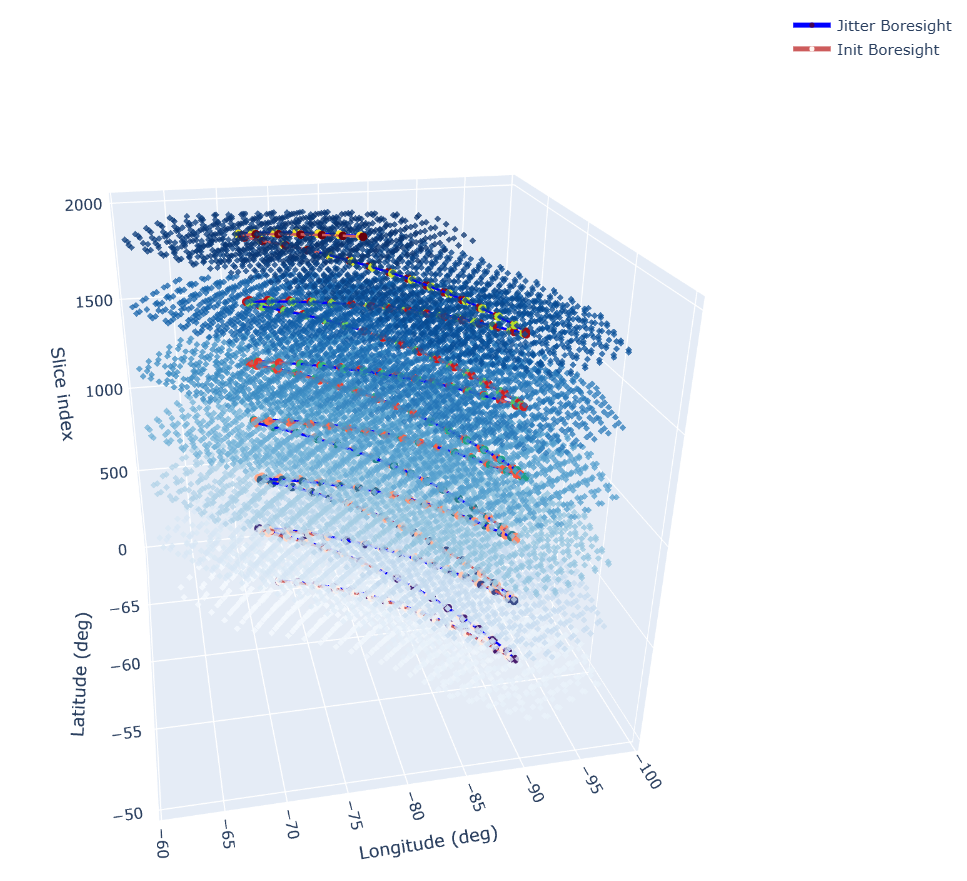
\includegraphics[width=0.75\textwidth]{Updates/figures/jitter_html.png}
    \caption{Pointing jitter boresight residuals.}
    \label{fig:boresight_html}
\end{figure}

After the ml mapmaker, the resulting map look like:

\begin{figure}[h!]
    \centering
    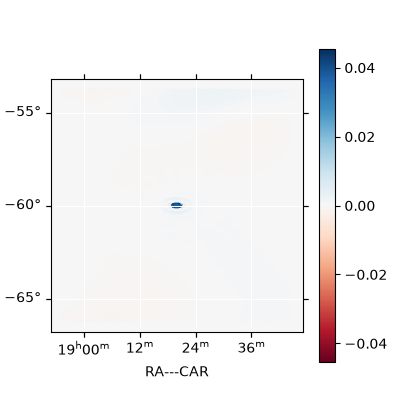
\includegraphics[width=0.75\textwidth]{Updates/figures/simple_nojitter_mlmap_I.png}
    \caption{Output I map of ML mapmaker with no jitter.}
    \label{fig:mlmap}
\end{figure}

This work has been a good proof of concept for implementing a pointing jitter, however, there are major limitations to this setup for simulating a realistic LAT scan. First, this telescope/focal plane objects are not representative of a realistic LAT. Second, other elements of the simulation like noise, atmosphere, etc. are not included in a realistic manner. It would see that the best way to proceed is to learn how the realistic LAT sims are actually run and incorporate my pointing jitter into that framework.




\pagebreak
% \bibliography{bib}

\end{document}
